\question \textbf{Tree topology}

A rooted phylogenetic tree can have three topologically different trees when $m$ is 3.

\begin{parts}

\vspace{0.1 in}

%% (a)
  \part  Fill the labels A, B, or C to satisfy three topologically distinct trees.
  
\begin{figure}[H]
      \centering
      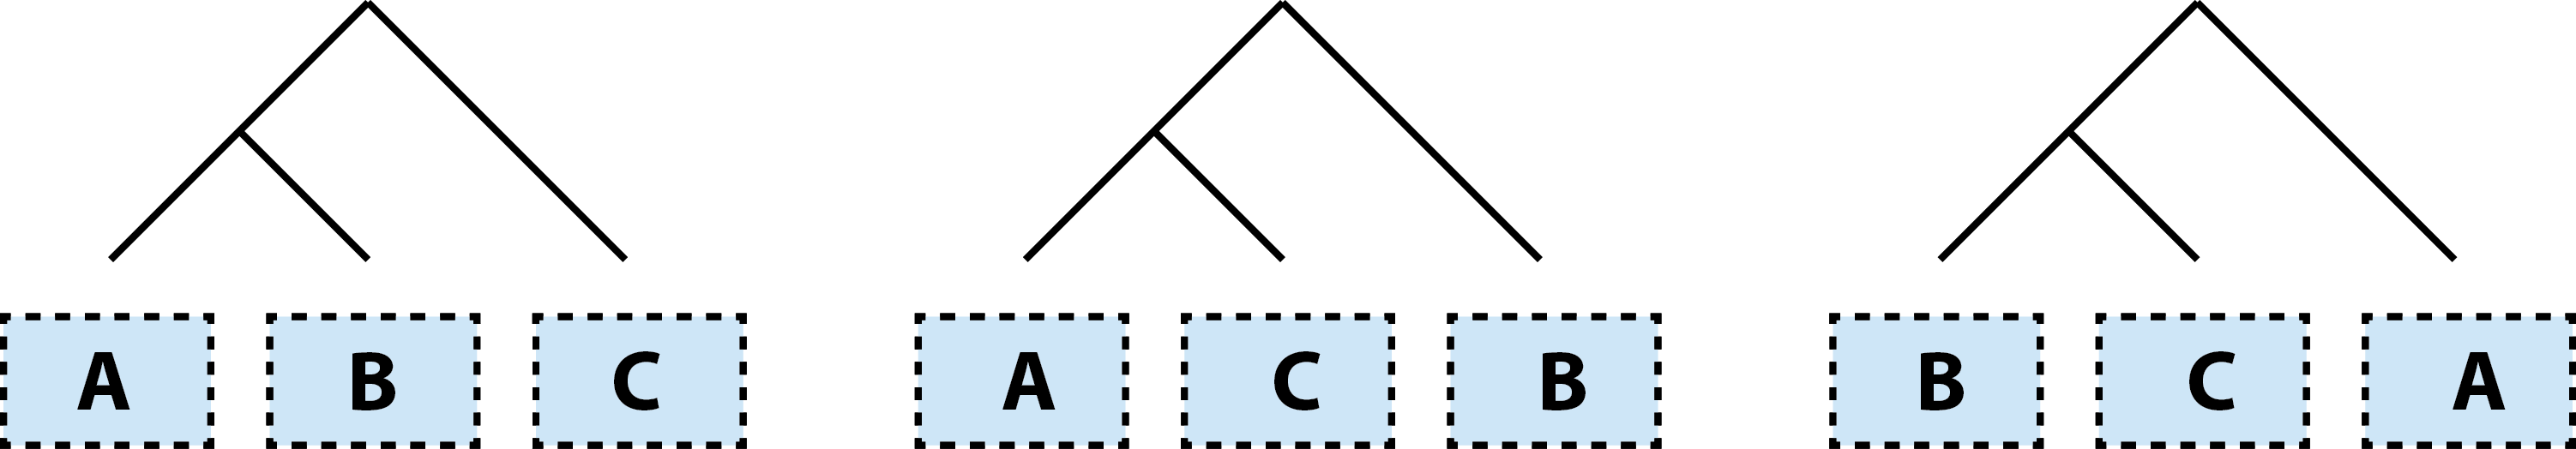
\includegraphics[width=0.7 \textwidth]{fig09/tree_topology_solution.png}
\end{figure}

\end{parts}

